\documentclass[11pt]{article}
\usepackage{color}
\usepackage{authblk}%allows footnote format for authors
\usepackage[letterpaper, margin=1in]{geometry} %package that allows changes in margins and header/footers
\usepackage[numbers,sort]{natbib}
\usepackage{amsmath}
\usepackage{rotating}
\usepackage{adjustbox}
\usepackage[english]{babel}
\bibliographystyle{ieeetr}
\newcommand{\mbh}[1]{\textcolor{orange}{ \emph{\scriptsize  #1}} } %creating command for Matt's comments
\newcommand{\lwang}[1]{\textcolor{red}{ \emph{\scriptsize  #1}} } %creating command for Li's comments
\newcommand{\gmj}[1]{\textcolor{blue}{ \emph{\scriptsize  #1}} } %creating command for Garrett's comments

\title{Review: Crop adaptation through introgression from wild relatives}

\author[1]{Authors: Garrett M. Janzen}%author information
\author[1]{Li Wang}
\author[1,*]{Matthew B. Hufford}
\affil[1]{Department of Ecology, Evolution, and Organismal Biology, Iowa State University, Ames, Iowa, USA}
\affil[*]{Correspondence: mhufford@iastate.edu (M.B. Hufford)}
\date{}

\begin{document}



\maketitle

%Short Research reviews should be in the range 3500–4000 words, with up to 40 references and 6 figures/tables.


The process of domestication was one thought to be rapid and geographically-constrained, with origin from a wild relative within one or more geographically-defined centers followed by expansion to the modern-day extent of cultivation.
However, archaeological and genetic evidence are revealing that domestication is more often temporally-protracted and multiregional \cite{brown2009complex}.
This new conception of domestication emphasizes the role of gene flow of beneficial alleles into domesticating populations from sympatric, locally-adapted wild relatives, a process known as adaptive introgression.



Adaptive introgression has three components: hybridization between two genomes, backcrossing to one of the parents, and selection on different recombinant genotypes with progressively diminished linkage drag \cite{barton2001role, Feuillet200824}.
In the case of adaptive introgression into domesticated crops, crop/wild hybrids backcross to the domesticate and adaptive genomic regions are retained and increase in frequency in the population as recombination separates desirable alleles from neighboring maladaptive alleles, which are selected against and lost.
Much attention has been given to the risk of natural introgression of transgenes from domessticated crops into wild relatives (for a review, \cite{stewart2003transgene}), or the history, utility, and methods of breeding programs designed to introgress desired traits from wild relatives (for a review, \cite{zamir2001improving, tanksley1997seed, hajjar2007use}), but recent tools and methods have been employed to detect genome-wide patterns of introgression in a number of species, granting insights into the prominence of adaptive introgression in crop domestication.


In this review, we will: 1) briefly describe these methods and provide a summary of their application for detecting crop-wild introgression, 2) review evidence supporting the hypothesis that wild-to-crop introgression has conferred local adaptation, 3) consider how the prevalence of this introgression alters traditional concepts of domestication, and 4) describe future advances in both basic and applied genetics that can be made through the study of introgression in agroecosystems.

\section*{Introgression methods and their applications}

The recent availability of genome-wide resequencing and reduced-representation genotyping (\emph{e.g.}, GBS and RAD-Seq) data, combined with new analytical methods, has facilitated comprehensive study of introgression across a number of species (\textbf{Table 1}).

High-density marker data can be used with haplotype-based and other methods to assign specific genomic regions to a taxon of origin and to identify introgression across taxa \cite{Martin2015,Price2009,Lawson2012,pease2015,rosenzweig2016,geneva2015}.

The methods introduced here do not include those marginally estimating introgression\slash migration rate as a component in the complete demographic history, such as Approximate Bayesian Computation (ABC) \cite{beaumont2002}, diffusion approximations for demographic inference (dadi) \cite {gutenkunst2009}, sorts of isolation with migration model \cite{hey2004}, and the multiple sequentially Markovian coalescent (MSMC) \cite{schiffels2014}. 
The collection of methods described different layers of genetic variation: diversity and divergence, haplotype variation and phylogenetic relationships.
We focus here on analytical prospects and limitations and introduce only a few representatives of each category.

First, genomic regions of introgression in admixed populations were expected to show a low level of divergence from source population.
$F_{st}$ and $d_{XY}$, as well as derivates such as $G_{min}$ \cite{geneva2015} and $RND_{min}$\cite{rosenzweig2016}, are representatives of such statistics. 
The former two are insensitive to rare migrants, and are therefore poorer at detecting recent introgression, while the latter two overcome these disadvantages.
 
 \begin{equation}
    G_{min} = \frac{d_{min}}{d_{XY}}
 \end{equation}
 where $d_{min}$ is the minimum sequence distance between haplotypes in species X and Y.
 
 \begin{equation}
 	RND_{min} = \frac{d_{min}}{d_{out}}
 \end{equation}
where $d_{out}$ equals $(d_{XO} + d_{YO})/2$, the average sequence distance between each species and the outgroup ($O$).
In addition, $RND_{min}$ is sensitive to variable mutation rate, which is indicated by branch length to the outgroup taxa. 
 
These statistics were recently developed into several new statistics, such as $U_{A,B,C(w,x,y)}$, by adding the divergence between non-admixed populations ($A$) and source population ($C$) as a comparison to that between admixed populations ($B$) and source population ($C$)\cite{racimo2016}. 
This statistic summarizes number of sites, where one particular allele at frequency $y$ in source population has a frequency bigger than $x$ in admixed population ($B$) and a frequency smaller than $w$ in non-admixed population ($C$).
Similarly, $Q95_{A,B,C(w,y)}$ just sets a hard cutoff as $95^th$ percentile of allele frequencies in panel B \cite{racimo2016}. 
These two statistics were also designed to facilitate incorporatioon of two source populations (see details in \cite{racimo2016}).
 
 
Second, local ancestry reconvolution (also known as chromosome painting) can identify the genomic regions that come from different source populations \cite{schraiber2015}. 
Such methods usually take phased haplotypes as input, but MULTIMIX \cite{churchhouse2013} can take both phased and unphased haplotypes as input, unveiling the genomic ancestry from multiple source populations.


Third, ABBA-BABA statistics (also known as D-statistics) and their derivatives are widely applied to the search for signs of introgression in genomic patterns of shared derived variants between populations or species. 
Based on D-statistics, $\hat{f_{d}}$ \cite{Martin2015} and five-taxon D statistics \cite{pease2015} were developed to localize genomic regions under introgression. 
The former took allele frequencies from each population/species, and the latter detected introgression from the localized phylogenetic pattern.
Their strength in identifying specific regions enables one to explore the relationships between introgression and recombination rate/gene density/distribution of deleterious alleles and to better understand the genomic regions penetrable to foreign gene flow. 

Fourth, structure-related approaches are based on the popular software STRUCTURE \cite{pritchard2000}, which provides an estimate of the fraction of each individual's genome coming from each population. 
Many approaches in this respect have been developed.
Two of these, fineSTRUCTURE \cite{Lawson2012} and GLOBETROTTER \cite{hellenthal2014}, were selected as representations.
Different from STRUCTURE, fineSTRUCTURE not only identifies the number of populations, but also estimates the probability that genomic regions belong to one or the other populations. 
GLOBETROTTER is a development of fineSTRUCTURE that allows for tracing back to an unsampled source population and dating admixture events.

Application of these approaches across a number of plant and animal species suggests introgression can play an adaptive role. For example, introgression from ancient hominins (\emph{e.g.}, Neanderthals and Denisovans) to humans has been detected at loci controlling skin pigmentation, defense against pathogens, and toleration of high altitude (reviewed in \cite{Racimo2015}), introgression has conferred M\"{u}llerian mimicry across butterfly species (\cite{Heliconius2012}; introgression has spread insecticide resistance across mosquito species \cite{Norris2015}, and introgression across \emph{Mimulus} (\emph{i.e.}, monkeyflower) species has resulted in adaptation to pollinator preference and contributed to speciation \cite{Stankowski2015}.


\noindent{\textbf{Table 1:} List and brief description of recently developed methods and examples of empirical studies employing these methods.}

\noindent{\textbf{Figure 1}: Wing coloration patterns in \emph{Heliconius} and evidence for introgression across species based on Patterson's \emph{D}-statistic; adapted from \cite{Heliconius2012}.}


%\lwang{In this part, maybe better to incorporate this reference, Detection and Polarization of Introgression in a Five-Taxon Phylogeny; and a new method published this year RND\_min Powerful methods for detecting introgressed regions from population genomic data; I donot know if we should also include G\_min, that is the statistic we tried that didnot work well for us: A new method to scan genomes for introgression in a secondary contact model. I put the three in the bib file.}





\section*{Crop adaptation through introgression}


Over the last few years, several high-profile publications based on genome-wide data have documented introgression between crops and wild relatives outside putative domestication centers.
A history of introgression during diffusion appears to be the rule for crops rather than the exception.
Theory suggests that colonizing species will overwhelmingly be recipients of introgression from locally-adapted native species \cite{Currat2008}. Crops, given their frequent history of diffusion from defined centers of origin, are therefore potential recipients of adaptive introgression.
Recent empirical studies have revealed that introgression has occurred in many of the world's most important crops (\textbf{Table 2}).






\begin{enumerate}
\item{Maize:}






Maize (\emph{Zea mays} ssp. \emph{mays}) and the teosinte \emph{Zea mays} ssp. \emph{mexicana} (hereafter referred to as \emph{mexicana}) have long been the subject of research into adaptive crop/wild introgression.
Maize was domesticated from (\emph{Zea mays} ssp. \emph{parviglumis})approximately 9,000 years ago in the Balsas River Valley \cite{matsuoka2002single}.
From this domestication center, maize spread into the highlands of the Mexican central plateau, where it came into sympatry with wild \emph{mexicana}.
Introgression between \emph{mexicana} and Mexican highland maize has been reported based on evidence from both morphological data \cite {wilkes1977, lauter2004, doebley1984} and molecular analyses \cite{matsuoka2002, vanHeerwaarden2011, doebley1987, warburton2011, fukunaga2005}.
However, \citep{hufford2013} was the first to reveal evidence of adaptive introgression from \emph{mexicana} into Mexican highland maize.
The authors identified nine genomic regions which showed evidence of introgression from \emph{mexicana} to maize in both the HAMPMIX and the linkage model of STRUCTURE analyses with over seven sympatric population pairs among the nine pairs sampled.
Among the nine regions, three span the centromeres of chromosomes 5, 6, and 10, and one is located in the inversion polymorphism on chromosome 4, suggesting a significant role of genome structures restricting recombination in adaptive introgression.
By further characterizing the nine introgression regions, it is found that most regions contain long tracts of zero diversity, enriched with QTL linked with anthocyanin content and leaf macrohairs \cite{lauter2004} and over-represented with the SNPs demonstrating high association with temperature seasonality.
It was also revealed that in the growth chamber experiment, maize populations with introgression from \emph{mexicana} on chromosomes 4 (associated with QTLs controlling pigment density and macrohairs) and 9 (overlapped with QTLs for macrohairs) exhibited more macrohairs and greater pigmentation under the highland environmental settings than the populations with absence of introgression from \emph{mexicana}.
In summation, the introgressed alleles/haplotypes from \emph{mexicana} to maize conferred adaptation to highland habitats when maize migrated from Mexican lowlands.


Even though introgression from \emph{mexicana} to Mexican highland maize has been highly supported, it is yet unknown whether and to what extent such introgression could be found in other highland maize populations which are allopatric to \emph{mexicana}. 
A recent study \cite{Takuno2015} found little empirical or theoretical support for parallel highland adaptation in the Mexican and South American highland regions, which was explained partly by the difference in potential for adaptive introgression from wild relatives.
Adaptive SNPs in Mexican highland population were more likely located in the introgressed regions than those in South American highland populations.
Furthermore, the adaptive SNPs in the Mexican highland population were more likely also showing signatures of local adaptation in \emph{mexicana} and \emph {pulviglumis} populations than those South American highland population.
For these reasons, adaptive introgression from wild relatives may play a significant role in patterning the genetic differences of maize highland populations.


Several questions regarding \emph{mexicana} introgression yet remain.
Has the introgression from \emph{mexicana} spread to multiple highland populations? 
How do highland-adaptation traits differ among populations with and without introgression from \emph{mexicana}?
A recent study \cite{Wang2015manuscript} first utilized the ABBA-BABA statistics to evaluate the existence or absence of introgression from \emph{mexicana} to multiple highland populations, and then $\hat{f_{d}}$ statistic proposed by Martin et al. (2015) \citep{martin2015} were calculated to locate the introgressed loci. 
Figure \ref{fig:fd} shows the loess regression of $\hat{f_{d}}$ in $10kb$ non\-overlapping windows across chromosomes 4 and 5 in multiple comparisons. 
On chromosome 4 (Figure \ref{fig:fd}), Mexican highland (MexHigh) and Guatamalan highland (GuaHigh) exhibited strong evidence of introgression from \emph{mexicana}, and the peaks of distribution corresponded to the region identified in Hufford et al. (2013) \citep{hufford2013}.
The signal of introgression is absent for the other three populations.
On chromosome 5, the signals of introgression (the peak region of the distribution) are present in MexHigh, GuaHigh and Southwestern US Highland (SW\_US), but not the other two.
More details on the other chromosomes can be found in \cite{Wang2015manuscript}.
Overall, both analyses revealed that gene flow from \emph{mexicana} exists, not only to MexHigh maize, but also to GuaHigh maize, as well as to some individuals in SW\_US, but not to the Andes and South American lowland (SA\_Low) populations, suggesting different extent contributions \emph{mexicana} made to multiple maize highland landrace populations. 
The Andean maize, the population totally isolated from the occurrence of any teosinte species, underwent the severest historical bottleneck, as a population in the front wave of the serial founder effects. 
%The stronger genetic drift introduced by the smaller historical population size increased homozygosity but reduced the heterozygosity of the population, and it also extended the length of homozygosity.
The high frequency of deleterious alleles caused by stronger genetic drift in the Andes population, together with the reduced efficiency of selection against deleterious sites, contributes to the observed higher mutation load in the well-isolated maize population.
Although it is clear that the absence of introgression from wild relatives provided fewer genetic resources for highland adaptation (making the highland adaptation in the Andes unique), it is yet unknown whether or not being out of reach of wild relatives is a reason for reduced fitness in the Andes population.
Furthermore, the question of whether convergent evolution occurs between populations with and without introgression from wild relatives is a key topic for future studies in maize.









\item{Asian Rice:}




Introgression appears to have played an important role in the domestication history of rice.
The center of Asian rice (\emph{Oryza sativa}) domestication is not known with complete confidence, but genetic and archaeobotanical evidence points towards both the Yangzee Basin in China and the Ganges plains in India for \emph{O. sativa}, 8,200-13,500 years ago, from wild \emph{O. rufipogon}  \cite{oka2012origin, fuller2010consilience, ricepedia, molina2011molecular}\ or "the Asian form of \emph{O. perennis} complex" \cite{oka2012origin}\.
Asian rices readily hybridize both with other domesticated subspecies and with wild relatives (of which there are about twenty \cite{ricepedia}).
The high genetic diversity within \emph{O. sativa} is likely due to introgression with wild relatives both during domestication and upon the dispersal of \emph{O. sativa} into new environments and sympatry with new relatives \cite{second1982origin}.

In an attempt to categorize the varieties of Asian rice, \cite{khush2003classifying} performed isozyme polymorphism analysis (11 enzymes, 20 loci, 79 alleles) on 25,519 rice varieties.
The vast majority of the rice varieties fell into two groups; indica (73.45\%) and japonicas (23.02\%).
Japonica rice cultivars were likely domesticated first from wild rice populations in southern China, and indica cultivars later developed through hybridization of ancient japonica with new wild rice populations in south and southeast Asia \cite{Huang2012, londo2006phylogeography}.
However,about 1.26\% belonged to four other groups (and 2.27\% were indeterminate).
Some of the varieties from these other four groups most likely arose from hybrids of cultivated rice and \emph{O. rufipogon}.
Introgression of alleles between cultivated rices, as well as between cultivated and wild rices, is common \cite{oka2012origin, second1982origin, zhao2010genomic}\, and natural introgression from wild to domesticate is suspected (\cite{zhao2010genomic} calls for research into this possibility).
These rices often have blight resistance gene, likley imparted from the wild relative parent.
Several resistance genes (grassy stunt virus, bacterial blight, brown planthopper, blast) are known to have been introgressed from wild relatives into \emph{O. sativa} by researchers \cite{brar1997alien, khush1974inheritance}.
Some aus and rayada varieties retain characteristics of the putative wild parent.
Aus exhibits a sprawling growth pattern and easy-threshing grain.
Rayada is adapted to areas with longer periods of flooding, with heightened seed dormancy and photoperiod sensitivity (permitting harvest during times without standing water).
Aswina variety, adapted to growth in deepwater conditions with a short period of flooding, seems to be the result of hybridization between \emph{O. sativa} and deepwater-adapted \emph{O. rufipogon} populations.

In addition to investigative experiments, gene flow from wild relatives has been utilized to produce agronomic rice varieties.
Yatsen No. 1, for example, showed resistance to pests and diseases and adapted well to environmental conditions \cite{ting1933wild}\.
Several lines were derived from Yatsen No. 1, and went on to be utilized extensively in parts of China.





		
	

\item{Barley:}
		
Domesticated and wild barleys belong to the same species, \emph{Hordeum vulgare}, and are biologically capable of producing viable offpsring via hybridizaion \cite{von1995ecographical}.
Barley (\emph{Hordeum vulgare} subsp. \emph{vulgare}) is believed to have been domesticated at least twice, once from wild subsp. \emph{spontaneum} in the Fertile Crescent and once from subsp. \emph{spontaneum} var. \emph{agriocrithon} in Tibet roughly 10,000 years ago \cite{takahashi1955origin, badr2000origin, oka2012origin, azhaguvel2007phylogenetic, haberer2015barley}\, but many of the details of barley domestication are still disputed.


Variety \emph{agriocrithon} is genetically diverse, and is found throughout much of the range of barley.
Some have suggested that \emph{agriocrithon} may be the progenitor of six-rowed barley, the product of a hybridization between eastern and western cultivated barley, or a wild-domesticate hybrid \cite{staudt1961origin, zohary1959hordeum, murphy1982origin}\, but \cite{azhaguvel2007phylogenetic}\ dispute these theories, suggesting instead that it arose from ssp. \emph{spontaneum}, perhaps more than once (in Israel as well as in Tibet).
Presently, the distribution of \emph{spontaneum} consists of the Mediterranean, the Middle-East, and west-central Asia, while other barley wild relatives inhabit Asiatic regions (including Tibet) more broadly \cite{nevo2010drought, harlan1995living, CWR}\.
These wild relatives inhabit regions spanning such abiotic clines as temperature, precipitation, soil type, and altitude, as well as biotic clines \cite{nevo2010drought}.


There has been little genetic investigation into spontaneous barley/\emph{spontaneum} hybrids \cite{ellstrand2003dangerous}\.
Barley/\emph{spontaneum} hybrids are fertile, and morphologically intermediate (putatively hybrid) barleys are found when wild and domesticated barleys are grown in sympatry, but hybrids of other wild relatives generally exhibit greatly diminished fertility \cite{ellstrand2003dangerous, harlan1995living}\.
Even when the two are not grown immediately adjacent to one another, introgression from wild to domesticate has been shown to happen over distances of more than a kilometer \cite{hillman2001new}.


The barley domestication process has reduced the number of alleles in the domesticate to only 40\% of that found in wild barley, though there remains a great deal of phenotypic diversity among the wild barleys \cite{ellis2000wild}\.
Wild-domesticate breeding experiments have shown that wild barleys have alleles for several important agronomic phenotypes, including powdery mildew resistance \cite{dreiseitl2017heterogeneity}, brittleness, flowering time, plant height, lodging, and yield \cite{von2006ab,handley1994chromosome}\.
The authors of \cite{Poets2015} used STRUCTURE to look for patterns of introgression from wild relatives in a dataset of 803 landraces.
The authors found a high amount variability in the amount of contribution from wild relatives, as well as its location in the genome, within barley populations.
This is indicative of contribution from numerous wild populations.
Furthermore, the authors find that wild introgression contribution is generally greatest from geographically-proximate populations, and that introgressed regions might be combined from geographically-separate wild populations.
Low linkage disequilibrium and small blocks of identity by state indicate that these introgressed regions are old, perhaps dating back to the beginning of domestication.
As landraces and nearby wild relatives share similar genomic sequences, the introgressed regions that are exclusive to that landrace are more more likely to contain adaptive alleles. 


The barley domestication process has reduced the number of alleles in the domesticate to only 40\% of that found in wild barley, though there remains a great deal of phenotypic diversity among the wild barleys \cite{ellis2000wild}\.
Wild-domesticate breeding experiments have shown that wild barleys have alleles for several important agronomic phenotypes, including brittleness, flowering time, plant height, lodging, and yield \cite{von2006ab,handley1994chromosome}.






















\item{Sunflower: }

The common sunflower (\emph{Helianthus annuus}) shows evidence of domestication in eastern United States \cite{harter2004origin, wills2006chloroplast}\, with additional evidence of a possible second origin of domestication in Mexico \cite{lentz2008sunflower}\.
Pre-Columbian \emph{H. annuus} distribution spanned much of the Great Plains, from what is now north-central Texas up to and through Montana and North Dakota (see figure 1 of \cite{whitney2010adaptive}).
Domesticated sunflower has long lived in sympatry with wild relatives like \emph{H. petiolaris} and \emph{H. bolanderi} and forms stable hybrid populations \cite{schwarzbach2002likely, rieseberg1988molecular, welch2002patterns}\.
Many wild sunflowers are locally-adapted, and weedy hybrid populations share these adaptations \cite{kane2008genetics}.
However, the most striking example of adaptive introgression within \emph{Helianthus} is that of the cucumberleaf sunflower, \emph{H. debilis} ssp. \emph{cucumerifolius}.
Cucumberleaf sunflower is endemic to south-central Texas, and exhibits several adaptations to the region.
Introgressive hybridization imparted locally-adapted alleles from \emph{H. debilis} to \emph{H. annuus} via introgressive hybridization \cite{heiser1951hybridization}. 
These introgressed hybrids formed a new lineage of sunflower (\emph{H. annuus} ssp. \emph{texanus}, \emph{H. a. texanus} hereafter) which displays \emph{H. debilis}-like traits adaptive to south-central Texas climate and ecology.
These adaptive \emph{debilis}-like traits include resistance to herbivorous pests and an increased branching plant architecture, as well as higher overall fitness than \emph{H. annuus} (as measured by higher seed production)\cite{whitney2006adaptive}.
Although H. annuus and \emph{H. a. texanus} are interfertile, \emph{H. a. texanus} displays persistent phenotypic differences from \emph{H. annuus} \cite{rieseberg2007hybridization}.


The genome of the common sunflower has been greatly influenced by introgression from wild relatives, due to both natural outcrossing events and concerted breeding efforts in crop improvement.
\emph{Helianthus} has several genes for downy mildew resistance, and each imparts resistance to one or more races of \emph{Plasmopara halstedii}, one of the most agronomically important diseases in sunflower cultivation \cite{cohen1973factors}\.
Some of these downy mildew resistence genes were found in wild relatives (including \emph{H. argophyllus}, \emph{H. tuberosus}, and \emph{H. praecox}) and have been successfully bred into modern \emph{H. annuus} \cite{miller1991inheritance}\.
PlArg, an allele found in wild silverleaf sunflowers (\emph{H. argophyllus}, inbred line Arg1575-2), confers resistance to all known (20 or more) races of downey mildew \cite{dussle2004pl}\, while others (Pl1-Pl11) are effective for one or more types \cite{rahim2002inheritance}\.
Silverleaf sunflower has also been the focus of drought resistance breeding efforts \cite{saucă2010introgression}\ and \emph{Phomopsis} resistance breeding efforts \cite{besnard1997specifying}.
\emph{H. annuus} shows signs of persistent introgressive hybridization with \emph{H. petiolaris} with evidence of positive selection driving some of the genetic differentiation between the two species \cite{yatabe2007rampant}.


Recent investigations into the history of \emph{Helianthus} introgression have implemented genomic methods.
\cite{Baute2015} analyzed transcriptome sequence variation on cultivated and wild \emph{H. annuus}, \emph{H. petiolaris}, and \emph{H. argophyllus}.
Using STRUCTURE, these authors found that introgressions from wild relatives can be found on every chromosome in at least one modern line, covering over 10\% of the genome.
Of particular note is the modern line RHA 274, a modern line which was bred with H. a. texanus in the 1970s to restore a branching plant body architecture, which allows the plant to produce pollen for a longer period of time, increasing seed production.
RHA 274 has several large introgression from \emph{H. a. texanus}, including one at the site of HaGNAT, the domestication gene associated with branching.
These introgressed regions are not found in the non-branching lines Sunrise and VNIIMK8931, further suggesting that the \emph{H. a. texanus} introgressed regions are causative.

































%The species \emph{H. annuus} is a versatile species, capable of adapting to a wide range of environments across the Americas, Europe, Asia, and Australia \cite{kane2008genetics}.
%This versatility may be due in part either to phenotypic plasticity or genetic adaptability \cite{maron2004rapid}.









%whitney2006adaptive
%"these results suggest that introgression of biotic resistance traits was important in the adaptation of H. annuus to central and southern Texas."
%fitness (seed production) high in texanus than in annuus
%identified two pests to which resistance was imparted and important
%Discussion points: 1. texanus has higher fitness than annuus in central texas.
%2. texanus shared traits more in common with debilis than with annuus (herbivore resistance)
%3. 2 of the three traits from point two above are important for adaptation to life in central south Texas.
%The authors ask why these pest-resistance genes have not spread further north beyond this range.  They are uncertain, but conjecture that negative pleiotrophic effects are at play.

%whitney2010adaptive
%"We demonstrate that introgression has altered multiple aspects of the H. annuus phenotype in an adaptive manner, has affected traits relevant to both biotic and abiotic environments, and may have aided expansion of the H. annuus range into central Texas, USA."
%This paper really does show that this case of natural introgression was adaptive.
%The companion paper (2006 Whitney) will likely show the same thing, but I haven't read it yet.

%scascitelli2010genome
%"long-term migration rates were high, genome-wide and asymmetric, with higher migration rates from H. annuus texanus into the two parental taxa than vice versa."
%"H. annuus texanus may serve as a bridge for the transfer of alleles between its parental taxa."
%"contradict recent theory suggesting that introgression should predominantly be in the direction of the colonizing species."

%rieseberg2007hybridization
%this is a very good review.  i think i should use it for the table.
%they also show that traits were imparted from debilis to texanus, and that these are adaptive.  i think they also show genetic evidence, but i'm not sure.













	\end{enumerate}
	Predictions regarding the likelihood of adaptive introgression in additional crops can be made through comparison of their centers of origin to both their current extent of cultivation and the distribution of wild relatives across environmental gradients (\textbf{Figure 2}).
	
	
	

	
	
	
	
	
	
	
	





\begin{table}
\centering
\begin{adjustbox}{width=1\textwidth}
\small
\label{my-label}
\begin{tabular}{|p{5cm}|p{5cm}|p{2.6cm}|p{2.6cm}|p{2.6cm}|l|}
\hline
Crop & Compatible Wild Relatives & Hybrids and/or Hybridization & Evidence of Crop Introgression & Evidence of Adaptiveness & Source \\ \hline \hline
Maize (\emph{Zea mays} subsp. \emph{mays}) & \emph{Z. m.} subsp. \emph{mexicana}, \emph{Z. m. } subsp. \emph{parviglumis} & X & X & X & \cite{hufford2013genomic} \\ 
\hline 
Asian Rice (\emph{Oryza sativa}) & \emph{O. rufipogon} & X & X & X & \cite{Huang2012} \\ 
\hline
Barley (\emph{Hordeum vulgare}) & \emph{H. v.} subsp. \emph{spontaneum} & X & X & X & \cite{Poets2015} \\ \hline
Sunflower (\emph{Helianthus annuus}) & \emph{H. argophyllus}, \emph{H. bolanderi}, \emph{H. debilis}, \emph{H. petiolaris} & X & X & X & \cite{rieseberg2007hybridization}\\ 
\hline
Cassava (\emph{Manihot esculenta}) & \emph{M. glaziovii} & X & X & X & \cite{bredeson2016sequencing} \\ 
\hline
Potato (\emph{Solanum tuberosum}) & many & X & X & X & \cite{johns1986ongoing} \\
\hline
Tomato (\emph{Solanum lycopersicum}) & \emph{S. pimpinellifolium} & X & X & X & \cite{rick1958role} \\
\hline
Olive (\emph{Olea europaea} ssp. \emph{europaea} var. \emph{sativa}) & \emph{O. e.} ssp. \emph{europaea} var. \emph{sylvestris} & X & X & & \cite{diez2015olive} \\ 
\hline
Soybeans (\emph{Glycine max}) & \emph{G. soja} & X & X &  & \cite{lam2010resequencing} \\ 
\hline
Common Bean (\emph{Phaseolus vulgaris}) & \emph{P. v.} var. \emph{aborigineus, P. v.} var. \emph{mexicanus} [[not in this source]]& X & X[[?not much]] &  & \cite{papa2003asymmetry} \\
\hline
Grapes (\emph{Vitis vinifera} subsp. \emph{vinifera}) & \emph{V. v.} subsp. \emph{sylvestris} & X & X &  &  \cite{myles2011genetic} \\
\hline
Sorghum (\emph{Sorghum bicolor} subsp. \emph{bicolor}) & \emph{S. b.} subsp. \emph{arundinaceum, S. b.} subsp. {drummondii} & X & X &  & \cite{aldrich1992patterns} \\
\hline
Wheat (\emph{Tritium monococcum, T. dicoccum, T. aestivum}) & \emph{T. m. boeoticum, T. dioccoides, T. urartu, Aegilops speltoides, A. tauschii} & X & X[[?hybrid origins]] &  & \cite{zohary1969wild} \\
\hline
\end{tabular}
\end{adjustbox}
\end{table}

\begin{figure}[h]
	\centering
	\includegraphics[width=17.35cm]{figure_outline.png}
	\caption{Map of the domestication centers of four crops and the distribution of their interfertile wild relatives, overlaying average annual precipitation.}
	\label{boxplot:map}
\end{figure}

\begin{figure}[h]
	\centering
	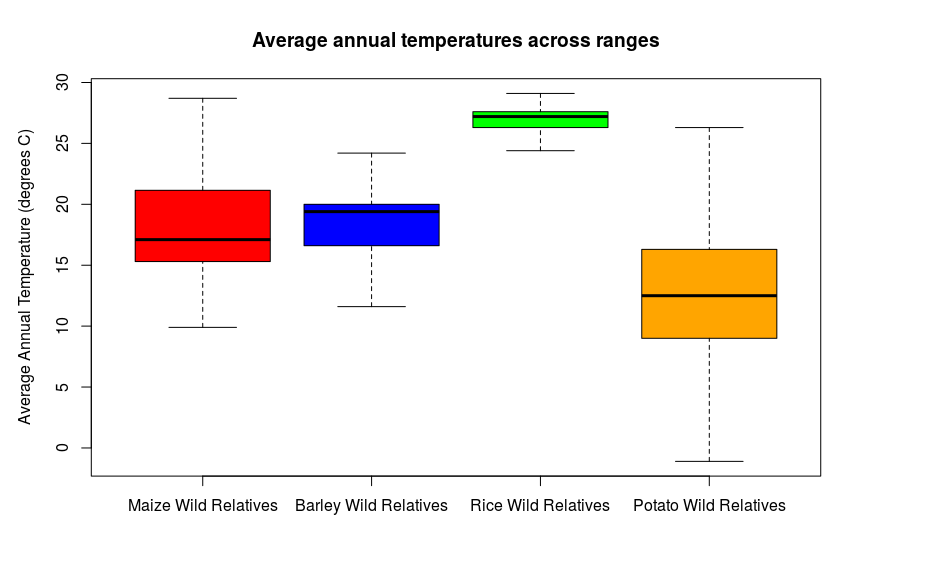
\includegraphics[width=17.35cm]{boxplot.png}
	\caption{The distribution of average annual precipitations experienced in the geographic home ranges of wild relatives interfertile with four crops}
	\label{fig:map}
\end{figure}



























\section*{Re-evaluating concepts of domestication}
A framework in which crops were domesticated from a single population or even a single species is, in several instances, an oversimplification.
A demography incorporating introgression from additional sources appears to be more correct for many crops.
With this in mind, certain aspects of crop evolution must be re-evaluated:

Estimates of the initial domestication bottleneck may be skewed when introgression is not considered.
Chromosomal regions experiencing introgression may have an altered effective population size ($N_e$) relative to non-introgressed regions depending on diversity within the donor taxon.
For example, introgression from wild taxa with historically high $N_e$ will lead to underestimates of the strength of the domestication bottleneck.


%\lwang{if the donor population has a relatively small population size, then the domestication bottleneck could be over-estimated.}\gmj{is the Kelley Harris, Rasmus Nielsen paper on Neanderthal genetic load in humans (the old CAMP paper) an example of this, Li?  I just want to make sure I understand.}
Estimates of the timing of domestication based on levels of sequence divergence may be affected when introgressed haplotypes are included.
%\lwang{It could be either inflated or underestimate,. It depends on the introgressed haplotype are more or less divergent from the wild progenitor, right?}


Loci under selection during domestication are often identified based on signatures of substantially-reduced nucleotide diversity in the domesticated taxon relative to the wild progenitor and high allele frequency differentiation between these taxa.
Introgression may alter these signatures and confound detection of domestication loci.
%\lwang{I donot quite understand this point. So, it is assumed that the introgressed haplotype has higher diversity, which renders difficulty to detect selection in such regions, right? But the case in maize is that even the introgressed haplotypes had higher diversity, but as selection has act long time on the region, the observed current diversity has already been reduced.}
%\gmj{It may not fit here perfectly, but you might consider a point about how crop-wild introgressions can also mask or obscure even the true progenitor species and center(s) of domestication.  The examples of potato and tomato domestication comes to mind; in potato, persistent and thorough interbreeding with a complex of wild relatives during domestication probably make it impossible to identify a single progenitor (if ever there was one), and in tomato, widescale recent introgression between two or three wild relatives confound attempts to identify which is the progenitor, and therefore the center of domestication as well.}












\section*{Future studies in crop-wild introgression}

New insights into domestication histories of crops are of potential value for the continued improvement of modern crops.
Continued research into this crop/wild introgression will prove valuable 


Additional study of introgression in agroecosystems could lead to advances in both basic and applied genetics.
Basic questions:
To what extent does the level of introgression across taxa depend on divergence time between donor and recipient taxa? %\lwang{maybe put alternative hypothesis here, or due to relative mutation load of the donor and recipient species?}
At what geographic scale does adaptive introgression occur? Is introgression frequently restricted to very local populations or is it often seen over broad geographic ranges? To what extent does this depend on the slope of environmental gradients such as temperature, precipitation, and elevation?%\gmj{Maybe not just geographical ranges, but also across environmental clines (e.g. temperature, precipitation, altitude, day lengh, etc.)?}
Can colonizing species served as bridges for gene flow between previously allopatric taxa? %\lwang{I feel the second and the third points could be combined. How the wild species could introgress into the allopatric landraces? Does domesticates serve as bridges?

Loci underlying the domesticated phenotype which may be beneficial targets for crop improvement can be more clearly identified by removing the confounding population genetic signal of introgression.
%\lwang{I am not quite clear with this point. It will be interesting to see that the domestication loci have further receive gene flow from the other wild relatives and it has not been purged out, as I think the domestication loci undergo strong positive selection, thus also strong purifying selection to dispel influx gene flow. Right?}
%\gmj{Removing the signal of introgression, is this more likely to uncover new and interesting domestication loci, or will it more likely reveal that some of the previously-identified loci of interest are not very interesting after all (as in, the identification of the introgression changes our understanding of the history of the locus and there is less evidence of selective pressures on it), or equally either case?  I hope that question made sense.}
Adaptive introgression that is clearly tied to a specific environment may include beneficial alleles that can be utilized in crop breeding.







\bibliography{bib_gj}

\end{document}


\end{document}


